\chapter{Richieste di informazioni da parte degli utenti}
\label{chap:informations}
I casi d'uso di uno strumento come questo assistente vocale potrebbero però \textbf{non fermarsi al mero indirizzamento di pazienti}. Infatti, potremmo plausibilmente aspettarci che gli utenti desiderino anche \textbf{ottenere informazioni di carattere medico} senza doversi per forza rivolgere ad un dottore.
\section{Enciclopedia medica del Ministero della Salute}
Pare ovvio sottolineare che le fonti delle informazioni riferite ai pazienti debbano essere \textbf{il più affidabili possibile}. Affidarsi a siti web come Wikipedia, per quanto comodo possa essere, è rischioso: le informazioni possono essere modificate da chiunque, anche e soprattutto persone poco qualificate.
Esiste però, in rete, una risorsa sconosciuta ai più, ma senz'altro interessante per i nostri scopi: l'\textbf{Enciclopedia Medica del Ministero della Salute}, accessibile sul sito del suddetto.
\begin{figure}[h]
    \begin{center}
        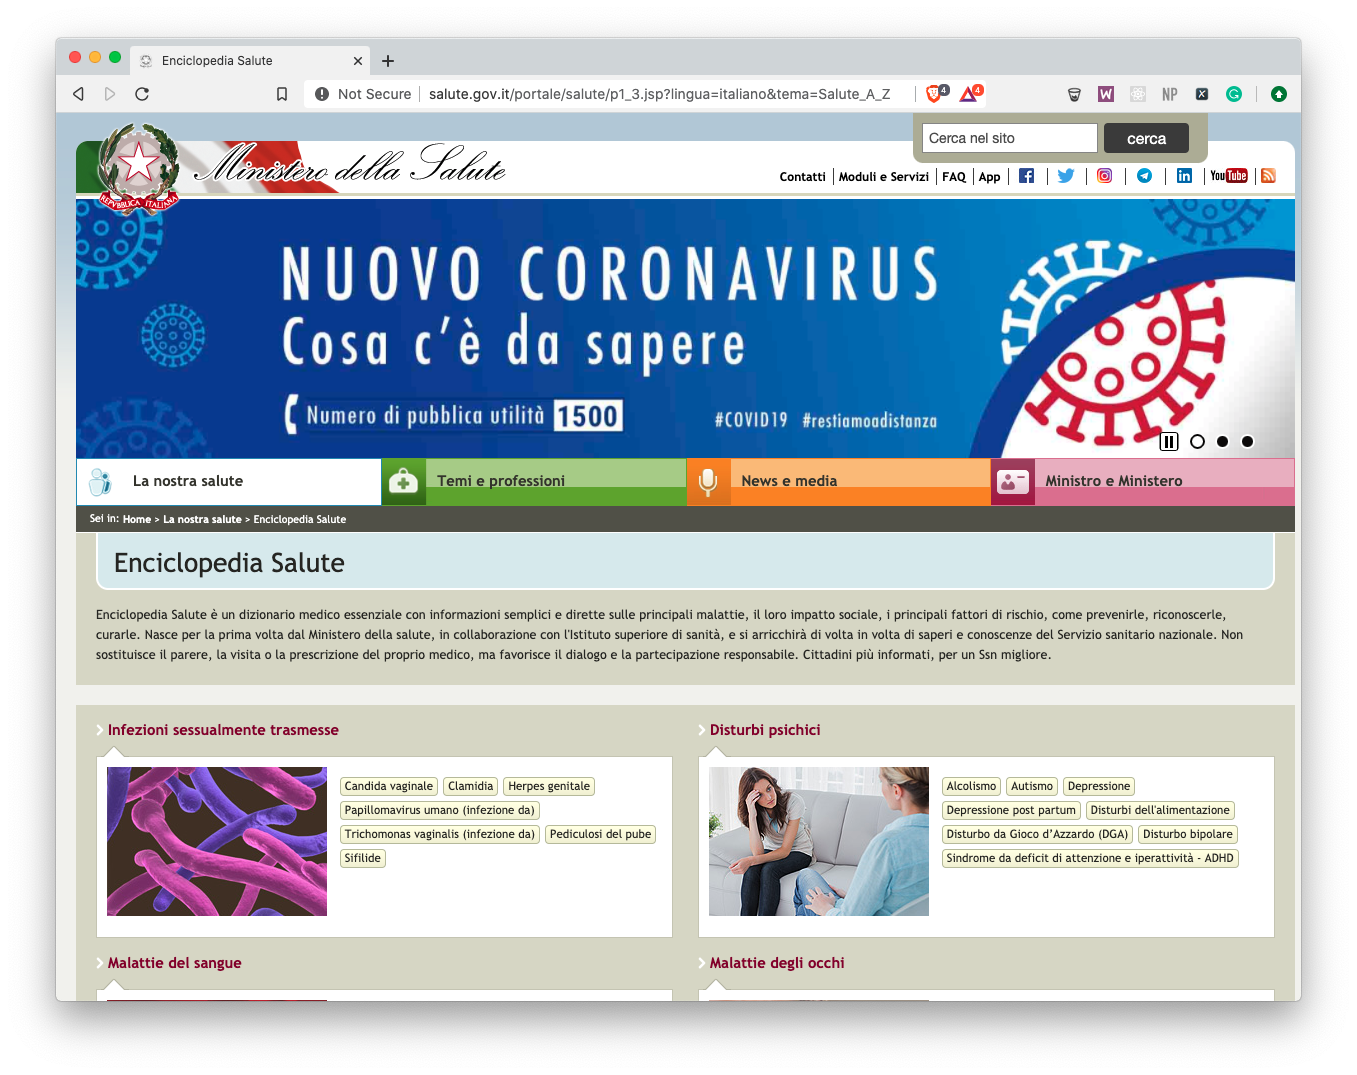
\includegraphics[width=0.8\columnwidth]{images/informations/MinSalute.png}
    \end{center}
    \caption{Enciclopedia della Salute}
    \label{fig:min-salute}
\end{figure}
\subsection{Utilizzo dell'enciclopedia}
Si potrebbe inizialmente pensare di trascrivere le informazioni dal sito: questo non è però certamente un approccio efficiente. Vorremmo allora automatizzare l'interazione con il sito web, in modo da ottenere i dati in modo autonomo. Viene, in nostro soccorso, il framework \textbf{Selenium}.
\subsubsection{Selenium}
Selenium è un framework nato con lo scopo di testare applicazioni web. È utilizzabile tramite un IDE proprietario, disponibile come estensione per Mozilla Firefox e Google Chrome, ma anche tramite scripts che interagiscono con \textbf{Selenium WebDriver}. Quest'ultimo accetta comandi in \textit{Selenese} o tramite una \textit{Client API}, e li trasmette ad un browser che ne raccoglie i risultati. È possibile definire questi scripts di testing in linguaggi diversi dal Selenese: dalla versione 2.0, Selenium WebDriver è totalmente implementato e supportato in Python, Ruby, Java e C\#. Durante il progetto abbiamo utilizzato la versione Python, installabile tramite PIP:
\begin{minted}[]{shell}
    pip3 install -U selenium
\end{minted}
Dopo l'installazione di Selenium, è ovviamente necessario anche un driver per interfacciarsi con il browser. Quello per Firefox è ad esempio \textit{GeckoDriver}, quello per Chrome \textit{ChromeDriver}. Ora, definire script per l'automazione di applicazioni web è semplice. Creando un oggetto tramite \texttt{webdriver.Firefox()}, avremo la possibilità di inviare comandi al browser ed interagire con la pagina web. Per fare ciò, ci basta selezionare un elemento tramite la sua classe CSS, il suo ID, un XPath: \texttt{find\_element\_by\_class\_name("nav-tabs")}. Fatto ciò, basta, ad esempio, chiamare il metodo \texttt{click()} sull'elemento. È anche possibile eseguire codice JavaScript: sul sito del Ministero della Salute, ad esempio, per disattivare il popup contenente le normative sui cookies sarà sufficiente eseguire \texttt{execute\_script("setPrivacy();")}.
\subsubsection{Approccio API}
Se i dati sul sito web cambiassero spesso, sarebbe molto utile definire un'API in modo da poter scaricare i dati al momento della richiesta. Tramite la libreria \texttt{http.server} è possibile definire una classe API (che estenda \texttt{BaseHTTPRequestHandler}), che ascolti una porta in attesa di richieste ed invii le risposte. Ad esempio, definendo un metodo \texttt{do\_GET}, esso verrà chiamato ogni qualvolta il server riceva una richiesta di tipo GET sulla porta designata. Definendo un oggetto \texttt{DataFetcher} che si occupi di gestire Selenium e l'interazione con la pagina, il metodo di risposta alla GET potrebbe essere così composto:
\begin{minted}[]{python}
def do_GET(self):
    parameters = parse_qs(urlparse(self.path).query)
    response = DataFetcher(parameters["query"][0])
    if response is not None:
        self.send_response(200)
    else:
        self.send_response(404)
    self.send_header('Content-type', 'application/json')
    self.send_header('Access-Control-Allow-Origin', '*')
    self.end_headers()
    if response is not None:
        self.wfile.write(json.dumps(response.get_query()).encode())
\end{minted}
Nella classe \texttt{DataFetcher}, dopo aver lanciato il WebDriver nell'\texttt{\_\_init\_\_}, basterà cercare il termine della query, e scorrere le tabs della pagina dell'enciclopedia. Essa è infatti divisa in sezioni come \textit{"Come si trasmette"}, \textit{"Sintomi"}, \textit{"Descrizione"}. Inviando quindi una richiesta tramite \textit{HTTPie}:
\begin{minted}[]{shell}
$ http "localhost:8000/?query=celiachia"

HTTP/1.0 200 OK
Access-Control-Allow-Origin: *
Content-type: application/json
Date: Fri, 19 Jun 2020 09:49:30 GMT
Server: BaseHTTP/0.6 Python/3.7.6

{
    "Cause": "La celiachia è una condizione multifattoriale, 
                [testo accorciato per motivi di stampa]",
    "Complicanze": "I soggetti affetti da celiachia non trattata 
                presentano un rischio maggiore di sviluppare complicanze, 
                [testo accorciato per motivi di stampa]",
    "Descrizione": "La celiachia, o malattia celiachia, è una malattia 
                permanente su base infiammatoria dell'intestino tenue caratterizzata 
                dalla distruzione della mucosa di questo tratto intestinale.
                [testo accorciato per motivi di stampa]",
    "Diagnosi": "Nei soggetti ad alto rischio di celiachia, per familiarità,
                 sintomi o per la presenza di una malattia frequentemente associata, 
                 [testo accorciato per motivi di stampa]",
    "Sintomi e segni": "I sintomi e segni della malattia sono estremamente
                 variabili per sede ed intensità.[testo accorciato per motivi di stampa]",
    "Terapia": "L’unica terapia attualmente disponibile per i soggetti celiaci
                 è la completa e permanente [testo accorciato per motivi di stampa]"
}
\end{minted}
\subsubsection{Approccio periodico}
Eseguire richieste all'API durante l'interazione con l'assistente vocale può generare \textbf{fastidiosi ritardi}. Siccome le informazioni sul sito web di cui sopra \textbf{non vengono aggiornate spesso}, può essere conveniente aggiornarle una volta al giorno e tenerle salvate in locale. Questo elimina del tutto i ritardi nel recupero delle informazioni, e ci permette un'integrazione \textbf{molto più efficace} in Mycroft: sapendo quali termini medici sono presenti nell'enciclopedia e quali no, il bot saprà già quali riconoscere e quali, invece, restituiranno un errore. Sfruttando come sempre Selenium, possiamo definire uno script utilizzando, in parte, il codice definito precedentemente. Basterà infatti chiamare la funzione \texttt{get\_query()} ciclicamente, una volta per termine disponibile nell'enciclopedia, ed accorpare tutti i risultati in un \textit{dictionary}, da salvare poi in JSON.
\begin{minted}[]{python}
def get_all(self):
    self.driver.get(MINISTERO_SALUTE_ENCYCLOPEDIA)
    fetched_data = {}
    aree = self.driver.find_elements_by_class_name("aree")
    for i in range(0, len(aree)):
        # This is kinda esoteric: the references on the DOM get changed on every refresh. 
        # So, we have to re-get them every time.
        aree = self.driver.find_elements_by_class_name("aree")
        aree[i].click()
        data = self.get_query()
        if data is not None:
            fetched_data[self.driver.title] = data
        self.driver.get(MINISTERO_SALUTE_ENCYCLOPEDIA)
    return fetched_data
\end{minted}
Una volta terminata l'esecuzione, ci basterà esportare i dati. Per fare ciò, utilizziamo due file: uno contenente le \textbf{informazioni}, uno contenente le \textbf{patologie conosciute}, da passare a Mycroft per il training di Padatious:
\begin{minted}[]{python}
data = df.get_all()
with open("informations.json", "w") as info_file:
    json.dump(data, info_file)
with open("locale/it-it/disease.entity", "w+") as entity_file:
    for name in data:
        entity_file.write(name+"\n")
\end{minted}
Fatto ciò, basterà definire un intent di Mycroft con frasi come \textit{"Dammi informazioni (sul|sulla|del|della|dei|sui) \{disease\}"}, dove \texttt{\{disease\}} indica un riferimento al file appena definito, contenente le malattie conosciute. È importante sottolineare come queste non siano strettamente richieste: un paziente potrebbe usare delle terminologie diverse. Per questo, vorremmo che il bot cercasse la malattia con \textbf{la miglior corrispondenza}, piuttosto che cercarla letteralmente. In questo modo, per esempio, "Tumore ai polmoni" sarebbe comunque ricollegabile a "Tumore del polmone". Una volta riconosciuta la malattia, Mycroft dovrà verificare \textbf{quali tipologie di informazioni possiede su di essa}, e chiedere all'utente di scegliere, domandando, ad esempio, \textit{"Cosa ti piacerebbe sapere? Scegli tra Sintomi, Cura, Terapia"}.
\begin{minted}[]{python}
# Let's find the most similar disease to what we've got
key, result = dictionary_searcher(
    message.data.get('disease'), self.informations)
# Tell the user the best match, and if it was wrong, say sorry
did_i_get_that = self.ask_yesno(
    "info.check_results", {"disease": key})
if did_i_get_that == "no":
    self.speak_dialog('sorry')
    return
# Let's create an array containing the choices of infos
self.possibilities = result
choices = ""
for choice in self.possibilities:
    choices = choices + choice + ", "
response = self.get_response(dialog='info.possibilities', data={
    "possibilities": choices})
info_key, info = dictionary_searcher(response, result)
self.speak_dialog(
    'info.speak', {"infos": info})
\end{minted}
Il bot è ora in grado di tenere conversazioni con i pazienti al riguardo di malattie, patologie, cure:
\begin{itemize}
    \item \textit{"Cosa sai dirmi sulla celiachia?"}
    \item \textit{"Ho trovato risultati per celiachia, è ciò che cercavi?"}
    \item \textit{"Esatto!"}
    \item \textit{"Cosa ti piacerebbe sapere? Scegli tra cause, complicanze, descrizione, diagnosi, sintomi e segni, terapia."}
    \item \textit{"Dimmi le cause."}
    \item \textit{"Ecco ciò che so: la celiachia è una condizione multifattoriale, [testo accorciato per motivi di stampa]"}
\end{itemize}
\section{Esempio di conversazione}
Riportiamo ora un esempio di conversazione realmente avvenuto. La conversazione è ascoltabile nei video disponibili sulla repo GitHub\cite{media:videos}.
\begin{itemize}
    \item \textbf{Utente:} \textit{Cosa sai dirmi sul tumore al fegato?}
    \item \textbf{Bot:} \textit{Il miglior risultato è Tumore del Fegato, è ciò che cercavi?}
    \item \textbf{Utente:} \textit{Esatto}
    \item \textbf{Bot:} \textit{Cosa ti piacerebbe sapere? Scegli tra Descrizione, Segni e sintomi, Cause, Diagnosi, Terapia, Prevenzione}
    \item \textbf{Utente:} \textit{Prevenzione}
    \item \textbf{Bot:} \textit{Questo è ciò che so: le uniche misure per ridurre le probabilità di ammalarsi di cancro al fegato sono l'adozione di stili di vita e misure di igiene che contrastino i fattori di rischio per questa forma tumorale}
\end{itemize}
\section{Aggiornamento dei dati}
Potrebbe configurarsi la necessità di verificare periodicamente il sito del Ministero della Salute in cerca di correzioni, modifiche, novità. Siccome la piattaforma è eseguita in ambienti Linux, uno straordinario strumento viene in nostro soccorso: \textbf{cron}. cron è un job scheduler per sistemi operativi UNIX. La sua struttura semplice permette di definire operazioni periodiche da svolgere in determinati istanti di tempo, all'interno di file detti \textbf{crontab} (\textit{cron table}). Ogni linea del crontab indica un'operazione da svolgere e gli istanti di tempo a cui farlo:
\begin{minted}[]{shell}
[min] [ore] [giorno] [mese] [giornodellasettimana] <comando da eseguire>
\end{minted}
Un asterisco sta ad indicare \textit{a tutti/e i/le ore/minuti/giorni...}. È anche possibile definire frazioni di intervalli di tempo: \texttt{*/2} verrà eseguito ad esempio una volta su due. Se quindi volessimo eseguire il fetching dei dati ogni notte, alle 02:00, basterebbe inserire nel crontab la seguente linea:
\begin{minted}[]{shell}
0 2 * * * cd hospital-triage-skill & python3 info_updater.py
\end{minted}
I più attenti potrebbero chiedersi perché non lanciare direttamente \texttt{python3 hospital-triage-skill/info\_updater.py}. Questo comando, apparentemente uguale al precedente, cela una grande differenza: non modifica la \textit{working directory} della linea di comando, che rimane la cartella home dell'utente. Essendo però i file salvati secondo un percorso relativo nel corso dello script Python, apparirebbero direttamente nella cartella home piuttosto che in quella del progetto.